\documentclass[12pt,a4paper]{report}
\bibliographystyle{plain}

\usepackage[utf8]{inputenc}
\usepackage{titling}
\usepackage{graphicx}
\usepackage{url}
\usepackage{appendix}
\usepackage[parfill]{parskip}
\usepackage{mathtools}
\usepackage{cite}
\usepackage[nottoc]{tocbibind}

\setcounter{secnumdepth}{0}

\newcommand{\pTwo}[1]{\frac{\partial^2}{\partial^2 #1}}
\newcommand{\inv}[1]{{#1}^{-1}}

\begin{document}

\title{Title}
\author{Martin Stølen}
\date{\today}

\clearpage

\section*{Problem Description}

\clearpage

\section*{Abstract}

In this project the wind simulator used in the snow simulator developed at
NTNU's HPC-lab will be implemented with the PETSc library. The goal of this
implementation is to use the GPU implementation of PETSc's solvers and to
compare the performance of these solvers with the previously implemented wind
simulation solvers. The performance of PETSc's GPU solvers will also be compared
with the performance of the solvers implemented in PETSc for multi-core CPU
systems to see if there is any gain from using the GPU implementations.

GPGPU programming is a recently developed area of high performance computing that
offers cost and energy efficient computing power by using many smaller and less
complex cores. Today GPGPU programming is mainly done using low level programming
APIs like CUDA and OpenCL. These APIs are considered to be challenging to
program with and may lead to complex software design.

PETSc is a library for high performance computing that implements matrix and vector
operations and a large selection of numerical solvers. PETSc is built to support
parallel programming with MPI and pthreads. In recent years PETSc has added
support for using the GPU with both CUDA and OpenCL. This enables usage of the
computational power of GPGPU programming for high performance
computing without having to program with low level APIs like CUDA and OpenCL.
The results show very good performance gains for using PETSc's GPU implementation.

\clearpage

\section*{Acknowledgements}

Thanks to Dr. Anne C. Elster for letting me use NTNU's HPC-lab which have been an 
invaluable workplace while I was working on the project. I'd also like to thank
Dr. Malik M. Zaki Khan for helping me get on the right track. Finally I want to
thank Christian Chavez for helping me with the workstation.
\clearpage

\tableofcontents
\clearpage

\listoftables
\clearpage

\listoffigures
\clearpage

\chapter{Introduction}



\section{Problem Description}

This project will implement a wind simulator in the HPC-lab's snow simulator 
using the PETSc library. PETSc was previously implemented in the CPU version
of the snow simulator by Mads Buvik Sandvei for his specialization project.
This project will implementing PETSc in the GPU version of the snow simulator
and utilize PETSc's GPU solvers in the wind simulation. 


\section{Outline}

Chapter 2 details the theoretical foundation material required for the wind
simulation. The chapter looks at the computational fluid dynamics model that is
used to simulate the wind and the assumptions made for the implementation. This
chapter also looks at the finite difference method, the topic of linear solvers
and PETSc will be introduced. Chapter 3 introduces the current version of the
HPC-lab's snow simulator. The history of the snow simulator is covered and the
structure of the code base is briefly outlined. Chapter 4 derives the
discretized mathematical expressions that have been implemented in the snow
simulator. Chapter 5 covers the details of the implementations that have been
done for this project. Chapter 6 presents the results of the implemented wind
simulation. Chapter 7 discusses the results and chapter 8 presents the
conclusions. Finally in chapter 9 possible future work to improve the
implementation is presented.

\clearpage

\chapter{Background}

This chapter will cover the mathematical background material for my problem. 
The first section of this chapter covers computational fluid dynamics (CFD) 
for the wind simulation as air can be modeled approximately as a fluid with 
zero viscosity and a density equal to one\cite{originalSnowThesis}.

The second section will cover partial differential equations and boundary value
problems, then go into further details about the Poisson equation which is 
solved as apart of the wind simulation.

The third section covers the finite difference method for creating systems of
linear equations approximating partial differential equations and will go into
details about the central difference and the discretized Poisson equation.

The fourth section covers the topic of linear solvers, explaining both direct
methods and iterative methods. This section goes into details about two direct
methods for solving systems of linear equations, Gaussian elimination and LU
decomposition and three iterative methods, the Jacobi method, Gauss-Seidel and
successive overrelaxation.

The fifth and final section will cover the Portable, Extensible Toolkit for
Scientific Computation, PETSc, which was used in the implementation.


\section{Partial Differential Equations}

A partial differential equation (PDE) is a differential equation with multiple 
unknown variables and their partial derivatives. PDEs can be used to model physical 
processes in multiple dimensions. 

\subsection{Boundary Value Problem}

A boundary value problem is a differential equation and a set of conditions for
the values on the boundary of the problem domain.

There are several different types of boundary conditions. If the values on the
boundary is given, then it is a Dirichlet boundary condition. If the normal
derivative to the border is given then it is a Neumann boundary
condition\cite{Kreyszig}.

\subsection{Poisson Equation}

In general, the Poisson equation is defined as 

$$\nabla^2 u = f$$

where $\nabla$ is the partial derivative and $u$ and $f$ are real or complex 
functions. In three-dimensional Cartesian coordinates, the Poisson Equation can 
be written as 

$$(\pTwo{x} + \pTwo{y} + \pTwo{z}) u (x, y, z) = f(x, y, z)$$


\section{Finite Difference Method}

The finite difference method (FDM) is a numerical method used to find an approximate 
solution to differential equations. It works by creating a discrete approximation 
of the derivative and using this approximation to write the differential equation 
as a system of linear equations.

There are different versions of the finite difference method.
\begin{itemize}
	\item Forward difference, $\Delta_hu(x) = u(x+h) - u(x)$
	\item Backward difference, $\nabla_hu(x) = u(x) - u(x - h)$
	\item Central difference, $\delta_hu(x) = u(x + \frac{1}{2}h) - u(x - \frac{1}{2}h)$
\end{itemize}

It is easy to see the connection of the forward difference and the definition of 
the derivative.

$$u'(x) = \lim_{h \to 0} \frac{u(x+h) - u(x)}{h}$$

We give $h$ a fixed, non-zero, value instead of having $h$ approach 0. Therefore 
the forward difference divided by $h$ approximates the derivative when $h$ is small.

$$u'(x) \approx \frac{u(x+h) - u(x)}{h}$$

The second order derivative can be approximated by applying the finite difference 
approximation to each term in the already derived expression for the approximation. 
For the central difference approximation another central difference approximation 
is applied to $u'(x + \frac{1}{2}h)$ and $u'(x - \frac{1}{2}h)$. This results in 
the following second order central difference approximation:

$$u''(x) \approx \frac{\delta_h^2u(x)}{h^2} = \frac{u(x+h) - 2u(x) + u(x-h)}{h^2}$$

When applied to higher dimensions, it is necessary to choose a value for h in 
each dimension. However we can simplify the resulting equation by choosing the same h. 
In three dimensions the approximation looks like this:

$$(\pTwo{x} + \pTwo{y} + \pTwo{z}) u(x, y, z) = \frac{\partial^2 u(x, y, z)}{\partial^2 x} 
+ \frac{\partial^2 u(x, y, z)}{\partial^2 y} + \frac{\partial^2 u(x, y, z)}{\partial^2 z}$$

$$\frac{\partial^2 u(x, y, z)}{\partial^2 x} \approx \frac{u(x+h, y, z) - 2u(x, y, z) + u(x-h, y, z)}{h^2}$$

$$\frac{\partial^2 u(x, y, z)}{\partial^2 y} \approx \frac{u(x, y+h, z) - 2u(x, y, z) + u(x, y-h, z)}{h^2}$$

$$\frac{\partial^2 u(x, y, z)}{\partial^2 z} \approx \frac{u(x, y, z+h) - 2u(x, y, z) + u(x, y, z-h)}{h^2}$$

This is also known as the 7-point stencil as illustrated in figure \ref{fig:7ps}.

\begin{figure}[ht]
	\center
	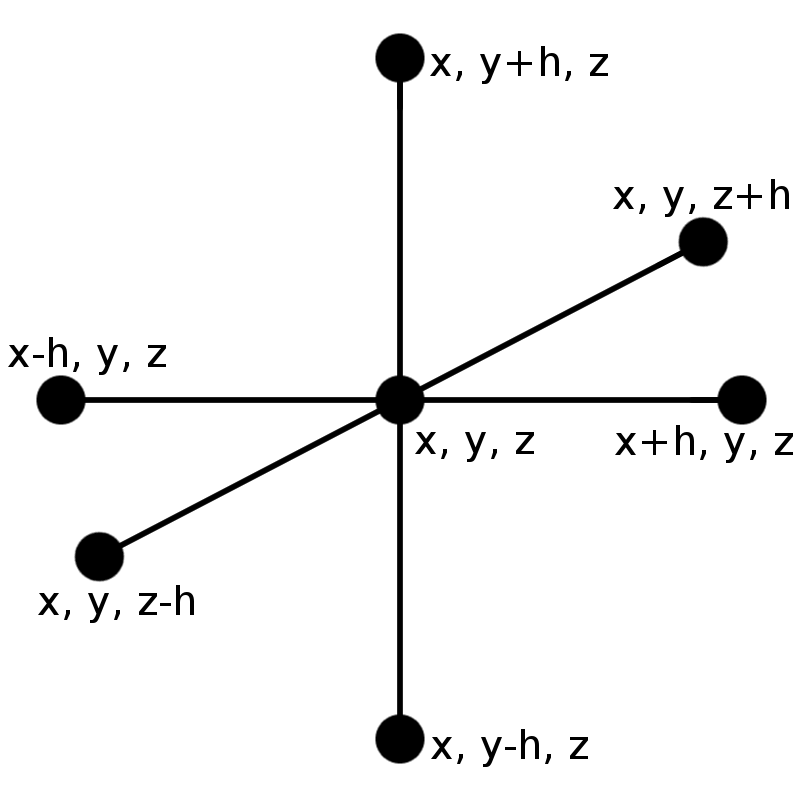
\includegraphics[width=0.5\textwidth]{images/7_point_stencil}
	\caption{7-point stencil}
	\label{fig:7ps}
\end{figure}

\subsection{Discrete Poisson Equation}

To apply the finite difference method to the Poisson equation with Dirichlet 
boundary conditions, problem domain is sampled in a finite number of points. 
The distance between the sample points, $h$, is the same as the fixed $h$ in the finite
differences method. Lets consider the two-dimensional Poisson equation $\nabla^2
u(x, y) = f(x, y)$. We use the central difference approximation to sample
$\nabla^2 u(x, y)$ at $n+1$ points in the $x$ direction and $n+1$ points in $y$
direction. We assume the dimensions of the domain goes from $0$ to $1$. The discretized 
grid is illustrated in figure \ref{fig:discgrid}.

\begin{figure}[ht]
	\center
	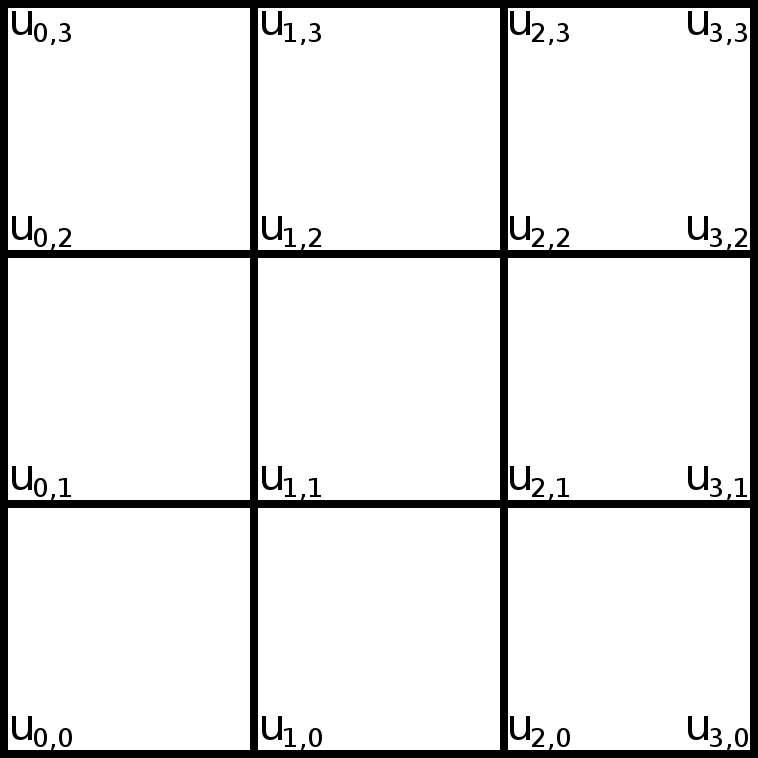
\includegraphics[width=0.6\textwidth]{images/2d_poisson_ex}
	\caption{Discretized grid with $n = 3$}
	\label{fig:discgrid}
\end{figure}

This gives $(n-1)^2$ internal points and the remaining points are boundary
points that have their values specified by the boundary conditions. The total
number of unknowns are therefore $N = (n-1)^2$.

$$h = \frac{1}{n}$$
$$x_i = ih, ~~~~ i = 0, 1, \dots, n$$
$$y_j = jh, ~~~~ j = 0, 1, \dots, n$$

We then denote the approximation of the value of $u(x_i, y_j)$ by $u_{i,j}$ and 
$f(x_i, y_j)$ by $f_{i,j}$

$$ (\nabla^2 u)_{ij} \approx \frac{u_{i+1,j} + u_{i,j+1} - 4u_{i,j} + u_{i-1,j} + u_{i,j-1}}{h^2} = f_{i,j} $$
$$ u_{i+1,j} + u_{i,j+1} - 4u_{i,j} + u_{i-1,j} + u_{i,j-1} = h^2 f_{i,j} $$

This creates a system of linear equations, that can be written on matrix form as
follows.

$$Ax = b$$

To create this linear system we have to create a global order for the
internal nodes to create the $x$ vector of unknowns. We use the natural
order, which means that we list the nodes along the $x$ direction first.

$$x_k = u_{i,j}, ~ k = (i-1) + (n-1) \cdot (j-1), ~ i, j = 1, 2, \dots, n-1$$

We can then assemble the matrix $A$.

$$
A = \begin{bmatrix}
 B & I & 0 & \cdots & 0 \\
 I & B & I &   & \vdots \\
 \vdots &   & \ddots &   & \vdots \\
 \vdots &   &   & \ddots & \vdots \\
 0 & \cdots & \cdots & I & B 
\end{bmatrix}
~~
B = \begin{bmatrix}
-4 & 1 & 0 & \cdots & 0 \\
 1 &-4 & 1 &   & \vdots \\
 \vdots &   & \ddots &   & \vdots \\
 \vdots &   &   & \ddots & \vdots \\
 0 & \cdots & \cdots & 1 &-4 
\end{bmatrix}
$$

$A$ is a $N \times N$ matrix, $B$ is a $(n-1) \times (n-1)$ matrix and 
$I$ is the identity matrix. Below we show how the matrix $A$ looks for 
$n$ = 3.

$$
A = \begin{bmatrix}
 -4 &  1 &  1 &  0 \\
  1 & -4 &  0 &  1 \\
  1 &  0 & -4 &  1 \\
  0 &  1 &  1 & -4
\end{bmatrix}
$$

%The vector $b$ is assembled from $h^2$, the function $f$, and the Dirichlet border conditions. 

%$$ b_k = h^2 \cdot f_{i,j} - u_{?} $$

%TODO: how is $b$ made


\section*{Linear Solvers}

A system of linear equations with $N$ unknowns can be written as 

$$Ax = b$$

where $A$ is a $N \times N$ matrix, and $x$ and $b$ are column vectors with $N$ 
elements each. $A$ and $b$ are known before hand, and we want to solve for $x$.

This can either be done with direct methods which compute the solution in a finite 
number of steps or by using an iterative method which iteratively improves an initial 
guess until we are satisfied. 

\subsection*{Direct Methods}

Direct methods are methods that solve the system of linear equations in a finite
number of steps. The conceptually simplest direct method is to find $\inv{A}$. 
There are different methods for finding the inverse of $A$, two of the most 
well known are Gaussian elimination, also known as Gauss-Jordan elimination, 
and LU decomposition, also known as LU factorization.

\subsubsection*{Gaussian elimination}

Gaussian elimination solves the system by performing row operations on the matrix 
$A$, to turn $A$ into the identity matrix. If these row operations are also performed 
on the vector $b$ then $b$ will be the solution vector when the Gaussian elimination 
is complete.

This method does not require you directly find $\inv{A}$, but finds the inverse 
indirectly. The combination of performing all the row operations is the same as 
multiplying with $\inv{A}$.

Gaussian elimination has O($n^3$) computational complexity, which means using 
Gaussian elimination is not feasible for solving equations with more than a few 
thousand unknowns with today's computing power.

Another problem with Gaussian elimination is that it is numerically unstable. 
When eliminating non-zero elements the algorithm may have to divide all the elements 
in a row with the value of the first coefficient on that row. If this number is 
close to zero any rounding error would be amplified.

\subsubsection*{LU decomposition}

The LU in LU decomposition stands for "Lower Upper". It works by factoring the 
matrix into the product of a lower and an upper triangular matrix. 

$$A = LU$$

To solve the linear system 

$$LUx = b$$

We first solve 

$$Ly = b$$

for $y$ by forward substitution. Then we solve 

$$Ux = y$$

for $x$ by backward substitution.

LU decomposition also has computational complexity O($n^3$). However LU decomposition 
is numerically stable, making it more suitable for a computer implementation.

\subsection*{Iterative Methods}

Iterative methods often start with a guess as to what the correct solution is, 
with the zero vector being a common choice for initial solution. Then they improve 
this solution by repeating a procedure multiple times, with each step 
giving an improved approximation to the solution of the problem. Iterative methods 
are not guaranteed to produce a correct solution in a given amount of steps. 

Iterative methods stop when a stopping criteria is met, normally when the difference 
between the right-hand side and the left-hand side or the change in the approximate 
solution is below a tolerance level given by the user. 

Another advantage of iterative methods is that we don't have to store the matrix 
$A$ because iterative methods don't depend on computing $\inv{A}$. This lowers 
the number of memory accesses that has to be performed. 

\subsubsection*{Jacobi Method}

The Jacobi method works by splitting the matrix $A$ into a diagonal matrix $D$ 
and the lower and upper triangular matrices $L$ and $U$. 

$$A = L+D+U$$

The matrix $D$ is diagonal and contains all the elements on $A$'s diagonal. $L$ 
is lower triangular and contains all the elements from $A$ below the diagonal. 
$U$ is upper triangular and contains all the elements from $A$ above the diagonal.

$$(L+D+U)x = b$$

The equation is then rearranged 

$$Dx = (b - (L+U)x)$$
$$x = \inv{D}(b - (L+U)x)$$

and the system is then solved iteratively by computing 

$$x^{(k+1)} = \inv{D}(b - (L+U)x^{(k)})$$

When parallelizing the Jacobi method we first write the element-based version:

$$ x_i^{(k+1)} = \frac{1}{a_{ii}} \Big( b_i - \sum_{j \neq j} a_{ij} x_i^{(k)} \Big), i = 1, 2, \ldots, n $$

Because the new value of each $x_i$ is independent of the new value for all the 
other elements in the $x$ vector, the Jacobi method is trivially parallel.

To converge this method requires the system to be strictly diagonally dominant[source],
meaning that for each row, the absolute value of the diagonal element must be
greater than or equal to the sum of the absolute value of the rest of the
elements on that row.

$$|a_{ii}| > \sum_{j \neq i} |a_{ij}|$$

The Jacobi method may converge even if this criteria is not satisfied, which is
the case with the Poisson equation.

\subsubsection*{Gauss-Seidel Method}

Gauss-Seidel works similarly to the Jacobi method, by splitting $A$ into $D$, 
$L$ and $U$. The main difference is how the equation is rearranged and the consequences 
when parallelizing the iterative solver. 

$$(L+D)x = b - Ux$$
$$x = \inv{(L+D)}(b - Ux)$$

$$x^{(k+1)} = \inv{(L+D)}(b - Ux^{(k)})$$

The value of $x^{(k+1)}$ has to be computed sequentially using forward substitution. 
There is no room for parallelization. Written in element-based form:

$$ x_i^{(k+1)} = \frac{1}{a_{ii}} \Big( b_i - \sum_{j < i} a_{ij} x_j^{(k+1)} 
- \sum_{j > i} a_{ij} x_j^{(k)} \Big),  i = 1, 2, \ldots, n $$

As we see from the first sum, the new value of $x_i$ depends on the new value of 
all previous elements in the $x$ vector.

It is possible to create a parallel implementation of Gauss-Seidel by changing
the order in which you calculate new $x$ values. This is known as Red-Black
ordering. The new ordering depends on the linear system you want to solve.

The convergence of the Gauss-Seidel method requires the matrix $A$ to be either
symmetric positive definite, or strictly diagonal dominant[SOURCE]. This method
converges faster than the Jacobi method, because it uses the new estimates for
$x$ found so far, in updating the value of the next element in the $x$ vector.

\subsubsection*{Successive Over-relaxation}

Successive over-relaxation is a modified version of Gauss-Seidel which gives
faster convergence. This method differs from Gauss-Seidel by introducing a
constant $\omega > 1$, which is called \emph{relaxation factor}. The system of
linear equations can be written as

$$ (D + \omega L)x = \omega b - \big( \omega U + (\omega - 1)D \big)x $$

$$ x = \inv{(D + \omega L)} \Big( \omega b - \big( \omega U + (\omega - 1)D \big)x \Big) $$

TODO: How to select a value for $\omega$ \\
TODO: Convergence


\section{PETSc}

PETSc is short for Portable, Extensible Toolkit for Scientific Computation. 
It contains various data structures and functions for 
high performance parallel computations. PETSc supports distributed 
memory systems with MPI, shared memory systems using pthreads or OpenMP as well 
as GPGPU computing using CUDA\footnote{\url{https://developer.nvidia.com/cuda-toolkit}} 
or OpenCL\footnote{\url{https://www.khronos.org/opencl/}}. PETSc is open source and distributed 
under the 2-clause BSD license\cite{petsc-web-page}.

\subsection{Programming Model}

PETSc is primarily written in C, but depends on certain Fortran libraries like 
BLAS\footnote{\url{http://www.netlib.org/blas/}} and LAPACK
\footnote{\url{http://www.netlib.org/lapack/}}. PETSc is written with an object-
oriented design pattern. There are object types for representing both data structures 
and solvers. Instead of accessing data directly, all manipulation of data structures 
uses functions that abstracts away the underlying implementation, there is no direct 
data access. PETSc's interface is designed based on the operations you perform on 
the data, rather than the data itself. This conceals complications as vectors being 
distributed to several machines running in parallel.

\subsection{Solvers}

PETSc implements a large number of parallel numerical solvers, for linear and 
nonlinear equations, as well as ordinary differential equations. For linear systems, 
PETSc implements both direct and iterative methods. The iterative methods implemented 
in PETSc are Krylov subspace methods, discussed in the section for linear solvers.
A complete list of the linear solvers implemented by PETSc can be found on the 
PETSc webpage\footnote{\url{http://www.mcs.anl.gov/petsc/documentation/linearsolvertable.html}}.

\subsection{GPGPU}

GPGPU stands for general purpose computing on graphics processing units. It was 
first implemented as a part of PETSc in 2010\cite{minden2010preliminary} by Victor 
Minden et al. PETSc can utilize CUDA through Thrust\footnote{\url{http://thrust.github.io/}} 
and Cusp\footnote{\url{http://cusplibrary.github.io/}} and OpenCL with ViennaCL
\footnote{\url{http://viennacl.sourceforge.net/}}. 

The changes required to have PETSc utilize the GPU is minimal. For the GPU 
implementation PETSc adds new subclasses of the vector and matrix classes that 
store the data on both the GPU and the CPU. Krylov solvers utilize GPU implementations 
of the functions defined for these classes.

To utilize the GPU the application programmer has to specify a GPU vector type 
for vectors and a GPU matrix type for matrices. This can either be done by using 
the \emph{VecSetType} and \emph{MatSetType} functions or by using the \emph{VecSetFromOptions}
and \emph{MatSetOptions} functions and specifying the type by adding \emph{-vec\_type} and 
\emph{-mat\_type} along with a GPU type on the command line during runtime. 

All Krylov subspace methods implemented in PETSc function on the GPU and require 
no data copies between the CPU and GPU while solving a system, with the exception
of the KSPIBCGS method (Improved Stabilized version of BiConjugate Gradient Squared),
which is not implemented for the GPU. This method requires direct access to the 
underlying data stored in the vectors and would require a complete rewrite to 
function on the GPU.

TODO: Preconditioners


\clearpage

\chapter{Previous Work}
\label{chap:prevwork}

This chapter will discuss previous work on the HPC-lab's snow simulator.

\section{Snow Simulator}

The snow simulator has been developed over several years by different students in 
the HPC-lab at NTNU. It simulates a finite number of snow particles and how they 
are affected by the wind and terrain. 

The snow simulator was originally developed  by Ingar Saltvik for his master
thesis \emph{"Parallel Methods for Real-Time  Visualization of Snow"}
\cite{originalSnowThesis}. Saltvik's implementation was  designed for multi-core
CPUs and achieved real-time performance for tens of  thousands snow particles
and unknowns for the wind simulation.

TODO: Insert figure of Saltvik's snow simulator

The snow simulator was later ported to the GPU by Robin Eidissen for his master 
thesis \emph{"Utilizing GPUs for Real-Time Visualization of Snow"}\cite{gpuSnowThesis}.
Eidissen's implementation achieved real-time performance with more than two million 
snow particles and four million unknowns in the wind simulation. 

TODO: Insert figure of the GPU snow simulator

TODO: Write about the other master theses and specialization projects that 
have worked on the snow simulator

%The following master theses have done work on the snow simulator:
%
%\begin{itemize}
%	\item Enhancing and Porting the HPC-Lab Snow Simulator to OpenCL on Mobile Platforms
%	\cite{openclSnowThesis}
%	\item Terrain Rendering Techniques for the HPC-Lab Snow Simulator\cite{snowTerrainThesis}
%	\item Enhancing the HPC-Lab Snow Simulator with More Realistic Terrains and Other Interactive Features
%	\cite{realisticSnowTerrainThesis}
%	\item Ray Tracing for Simulation of Wireless Networks in 3D Scenes\cite{rayTracingThesis}
%	\item OpenACC-based Snow Simulation\cite{openAccThesis}
%	\item Avalanche Simulations using Fracture Mechanics on the GPU\cite{avalancheThesis}
%\end{itemize}

\subsection{Overview}

TODO: Write a general overview of the different parts of the snow simulator

\subsection{Wind Simulation}

The wind simulation calculates the three dimensional wind velocity field through
computational fluid dynamics (CFD). The discretization method being used is the
finite difference method. The boundary conditions for the CFD problem is decided
by the terrain vertex data and the external wind velocity at the borders of the
domain. The external wind velocity can be set by the user at runtime. The system
is solved using a SOR- solver and the boundary conditions are satisfied by
adjusting cells that are next to obstacles.

\subsubsection{Implementation}

The wind simulator is implemented in CUDA and consists of eight kernels. Five of 
the kernels are used for simulation while the remaining three kernels are for 
visualization. The wind simulation uses the following data structures:

\begin{description}
	\item[wind\_vel,] a three dimensional array of float4 representing the wind 
	velocity field. At the end of the wind simulation step, the contents of this 
	array is moved to texture memory for efficient access by the snow particle 
	simulation. 
	\item[obstacle,] a three dimensional array of integers. The bits of each 
	integer indicate if the current cell or an neighboring cell contains an 
	obstacle. 
	\item[pressure,] a three dimensional array of floats containing the values 
	of the air pressure used in the projection step of the wind simulator. 
	\item[solution,] a three dimensional array of floats containing the solution 
	vector (right-hand side) for the Poisson equation. 
\end{description}

Each of the five simulation kernels handles a part of solving the momentum equation 
of the incompressible Euler equations.
\begin{description}
	\item[wind\_advect]
	\item[build\_solution2]
	\item[solve\_poisson2]
	\item[set\_boundary2]
	\item[wind\_project2]
\end{description}

The visualization kernels are used to visualize the data structures used when 
simulating the wind. These are the visualization kernels:

\begin{description}
	\item[make\_obs\_points,] visualizes the cells determined to be obstacles 
	for the wind from the terrain. 
	\item[make\_pressure\_points] colormapped points to visualizes the pressure 
	in the cells. 
	\item[make\_vel\_lines] visualizes the wind velocity field as field lines 
	colormapped depending on the magnitude of the wind velocity vector. 
\end{description}



\clearpage

\chapter{Implementation}

This chapter will look at the implementations done in this project. It will describe 
how PETSc was used to setup and solve the discrete Poisson problem for the wind 
simulation. 

\section{PETSc}

This section describes which PETSc functions were used and how they were used in 
the implementation of the linear solver\cite{petsc-user-ref}. 

\subsection{Setup}

The $DM$ object and $MatSetValuesStencil$ function are the primary functionality from 
PETSc used when creating the matrix $A$\cite{petsc-user-ref}. DM is short for 
Data Management and is used to manage the mapping between the distributed PETSc 
algebraic structures (Vec and Mat) and the structure of the mesh grids for the PDE. 
$MatSetValuesStencil$ handles the mapping from the physical coordinates of the 
internal nodes in the PDE matrix to their global ordering. 

The $DM$ object is used to get the process local domain of the matrix, 
making it possible to set the values of the matrix when it is distributed across 
different machines in a distributed memory system. $MatSetValuesStencil$ is used 
to set the values of the matrix.

To assemble the right hand side vector, $b$ the To create the mapping the function 
$DMDACreate3D$ was used.

\subsection{Solver}

The linear solvers used in PETSc are called KSP, which stands for Krylov subspace 
methods. 


\clearpage

\chapter{Results}

This chapter contains the test results for the PETSc port of the wind simulation. 
The first part will describe the hardware used in the workstation and the software 
used. It will also describe how the project and PETSc was compiled. The second part 
will look at the test results for the accuracy of the solver with a convergence 
test and the performance. 

\section{Setup}

This section will describe the compilation of PETSc and the snow simulator as well 
as the hardware and software of the workstation used for the tests in the next section. 

\subsection{PETSc}

PETSc was acquired from the PETSc Web Page\cite{petsc-web-page} as version 3.5.2. 
The version of the compilers used when configuring PETSc can be found in table 
\ref{table:workstation}.

For development, PETSc was configured with the following flags:
\lstset{language=bash}
\begin{lstlisting}
./configure --with-cc=gcc --with-cxx=g++ --with-fc=0 
--download-f2cblaslapack --download-mpich
\end{lstlisting}
Debugging is by default enabled by the PETSc configuration, therefore the debug 
flag is not being specified.

For performance tests, a PETSc configured with these flags were used:
\lstset{language=bash}
\begin{lstlisting}
./configure --with-cc=gcc --with-cxx=g++ --with-fc=0
--with-debugging=0 --with-precision=single
COPTFLAGS='-O3' CXXOPTFLAGS='-O3' 
--download-f2cblaslapack --download-mpich
\end{lstlisting}
For this configuration of PETSc debugging was disabled and precision was set to 
single. 

\subsection{Compilation}

\subsection{Workstation}

This project was only tested on one workstation. Table \ref{table:workstation} contains 
the specifications for the workstation used.

\begin{table}[h]
	\begin{center}
	\bgroup
	\def\arraystretch{1.2}
	\begin{tabular}{|l|l|}
		\hline
		\multicolumn{2}{|l|}{\textbf{Workstation hardware}} \\ \hline
		CPU & i7-3770 @ 3.4 GHz \\ \hline
		GPU & Nvidia GeForce GTX 980 \\ \hline
		Memory & 16 GB DDR3 1600 MHz \\ \hline
		Power supply & CORSAIR AX1200 \\ \hline
		\multicolumn{2}{|l|}{\textbf{Workstation software}} \\ \hline
		Operating system & Ubuntu 14.04 64-bit \\ \hline
		Nvidia driver & 343.22 \\ \hline
		CUDA toolkit & 6.5 \\ \hline
		g++ & 4.8.2 \\ \hline
		gcc & 4.8.2 \\ \hline
		PETSc & 3.5.2 \\ \hline
	\end{tabular}
	\egroup
	\end{center}
	\caption{Workstation specifications}
	\label{table:workstation}
\end{table}


\section{Tests}

TODO: Write about all the snow simulator configurations when doing these tests
Also write about what solvers were used by PETSc and which solver is used
by the default gpu snow simulator

TODO: When running the solver on the cpu the following command line arguments
are given: "\emph{-vec\_type standard -mat\_type aij}" and on the gpu:
"\emph{-vec\_type viennacl -mat\_type aijviennacl}".

The configuration options for the wind simulator allows for variation in the
external wind direction, speed and the resolution of the three dimensional wind
velocity field. For the scope of these tests only the resolution of the wind
velocity field is changed, while the external wind's speed and direction remains
unchanged for all tests. The resolution of the wind velocity field is denoted
as \{ x, y, z \}. The terrain used for the simulation tests is the height map of
Mount St. Helens with a size of 768x768. The external wind's speed is set to 1
and the direction is given by the unit vector \{1, 0, 0\}.

\subsection{Convergence Tests}

TODO: Write about the convergence

\subsection{Performance Tests}

\subsubsection{Time Distribution}

This test measures how the execution time of the wind simulation is distributed
between these key functions in the implementation:
\begin{description}
	\item[advect:] Performs the advection step of the wind simulation.
	\item[setupSolution:] Computes the right-hand side of the linear system.
	\item[setInitialGuess:] Sets the initial guess for the solver.
	\item[solve:] Solves the Poisson equation using a PETSc solver.
	\item[project:] Performs the projection step of the wind simulation.
	\item[windToGPU:] Moves the wind velocity field to texture memory for the
	snow particle simulation.
\end{description}

The solver chosen for this test is GMRES, this was specified with the command
line argument "\emph{-ksp\_type gmres}".

This test is performed for four different configurations for the resolution of
the wind velocity field:
\begin{description}
	\item[Configuration 1] $ \{ 32, 16, 32 \} $, the total number of internal
		points is 16384. Results are shown in figure \ref{fig:td_conf1}.
	\item[Configuration 2] $ \{ 64, 32, 64 \} $, the total number of internal
		points is 131072. Results are shown in figure \ref{fig:td_conf2}.
	\item[Configuration 3] $ \{ 128, 64, 128 \} $, the total number of internal
		points is 1048576. Results are shown in figure \ref{fig:td_conf3}.
	\item[Configuration 4] $ \{ 256, 128, 256 \} $, the total number of internal
		points is 8388608. Results are shown in figure \ref{fig:td_conf4}.
\end{description}

The results of the time distribution tests is the average execution time of each
key function after 100 frames of simulation.

\begin{figure}[ht]
	\center
	
	\begin{subfigure}{0.45\textwidth}
		\center
		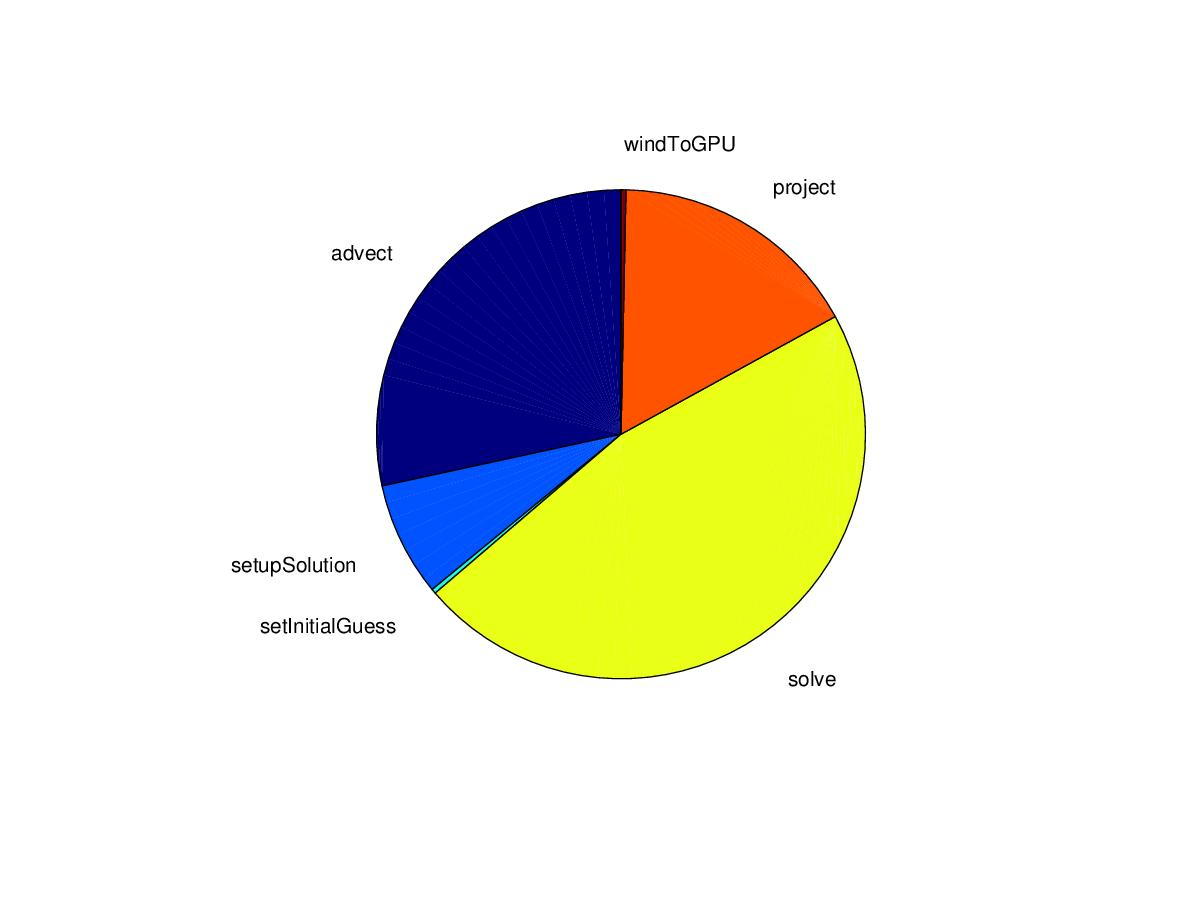
\includegraphics[width=1.0\textwidth]{results/data/td_conf1_petsc_gpu}
		\caption{PETSc on the GPU with OpenCL.}
		\label{fig:td_conf1_petsc_gpu}
	\end{subfigure}
	\begin{subfigure}{0.45\textwidth}
		\center
		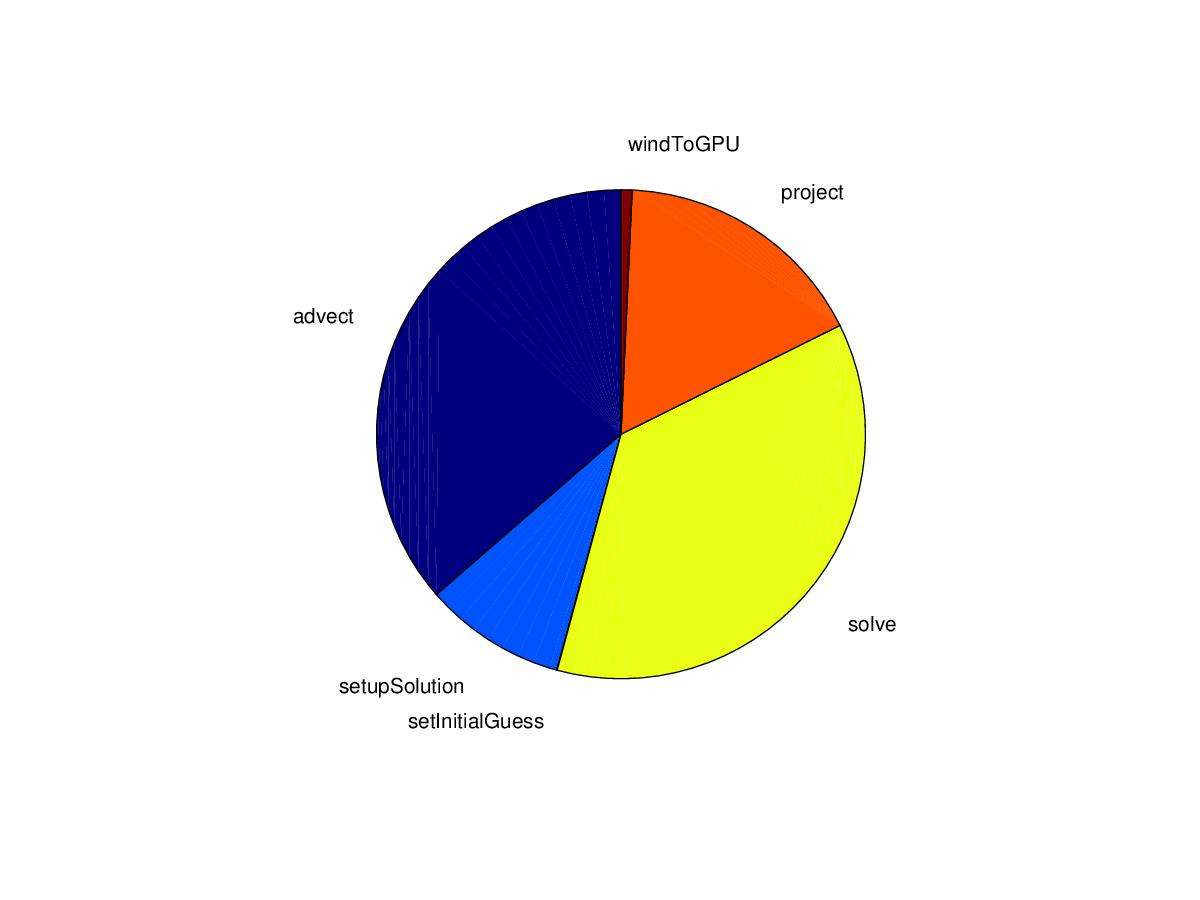
\includegraphics[width=1.0\textwidth]{results/data/td_conf1_petsc_cpu}
		\caption{PETSc on the CPU.}
		\label{fig:td_conf1_petsc_cpu}
	\end{subfigure}
	\caption{Time distribution of the execution time of the key functions
			with configuration 1}
	\label{fig:td_conf1}
	
\end{figure}

\begin{figure}[ht]
	\center
	
	\begin{subfigure}{0.45\textwidth}
		\center
		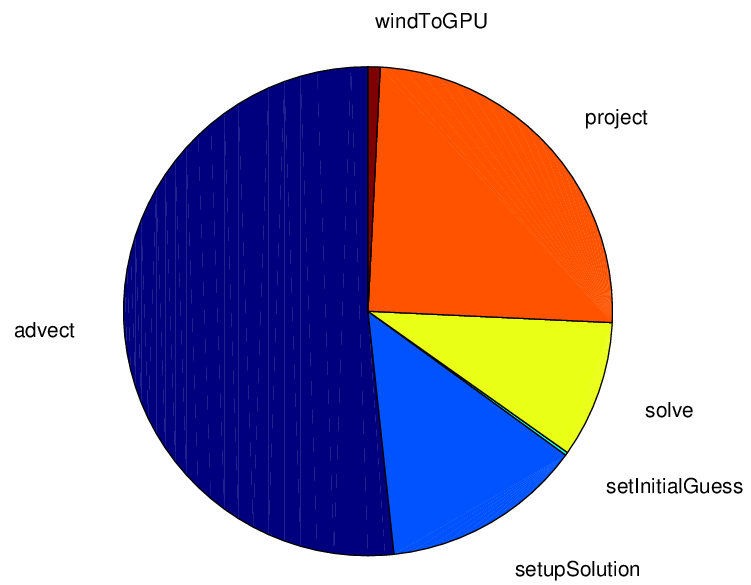
\includegraphics[width=1.0\textwidth]{results/data/td_conf2_petsc_gpu}
		\caption{PETSc on the GPU with OpenCL.}
		\label{fig:td_conf2_petsc_gpu}
	\end{subfigure}
	\begin{subfigure}{0.45\textwidth}
		\center
		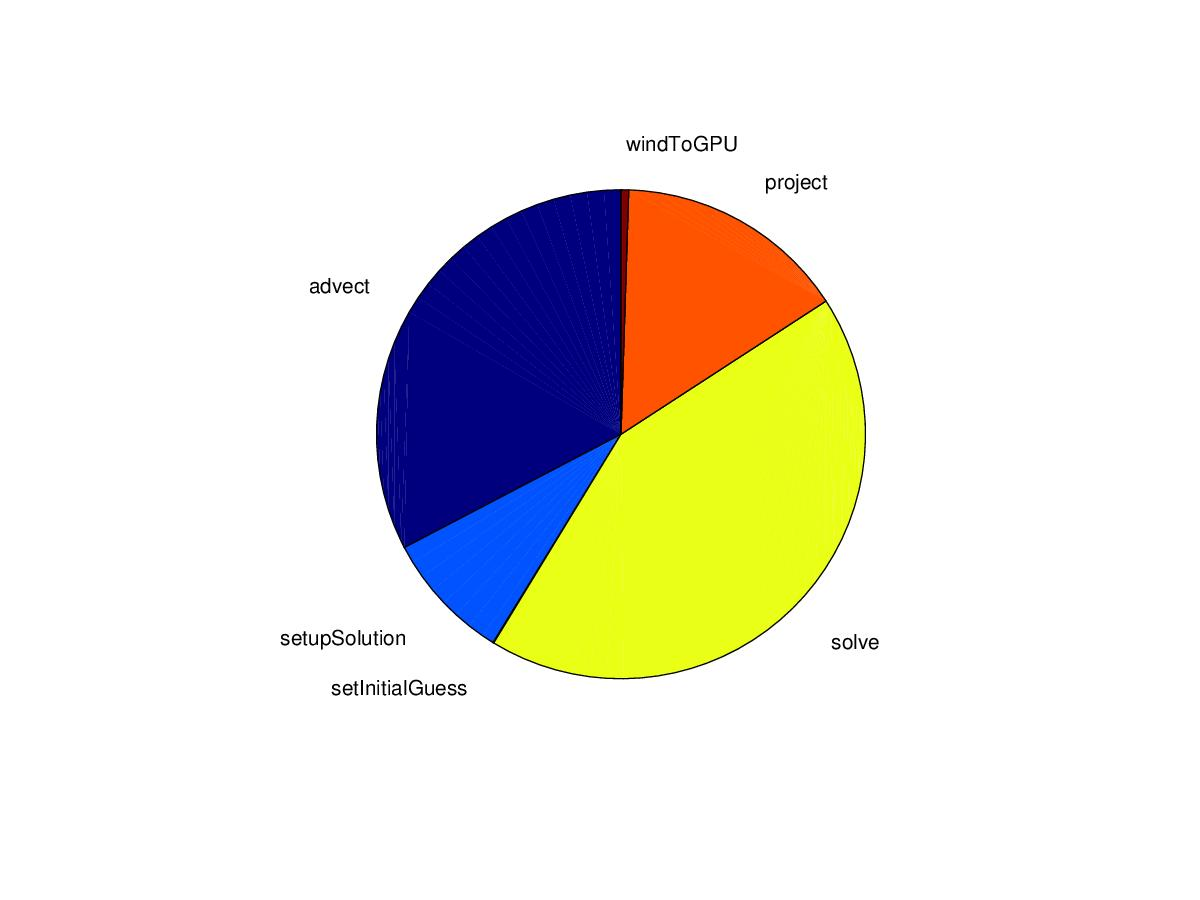
\includegraphics[width=1.0\textwidth]{results/data/td_conf2_petsc_cpu}
		\caption{PETSc on the CPU.}
		\label{fig:td_conf2_petsc_cpu}
	\end{subfigure}
	\caption{Time distribution of the execution time of the key functions
			with configuration 2}
	\label{fig:td_conf2}
	
\end{figure}

\begin{figure}[ht]
	\center
	
	\begin{subfigure}{0.45\textwidth}
		\center
		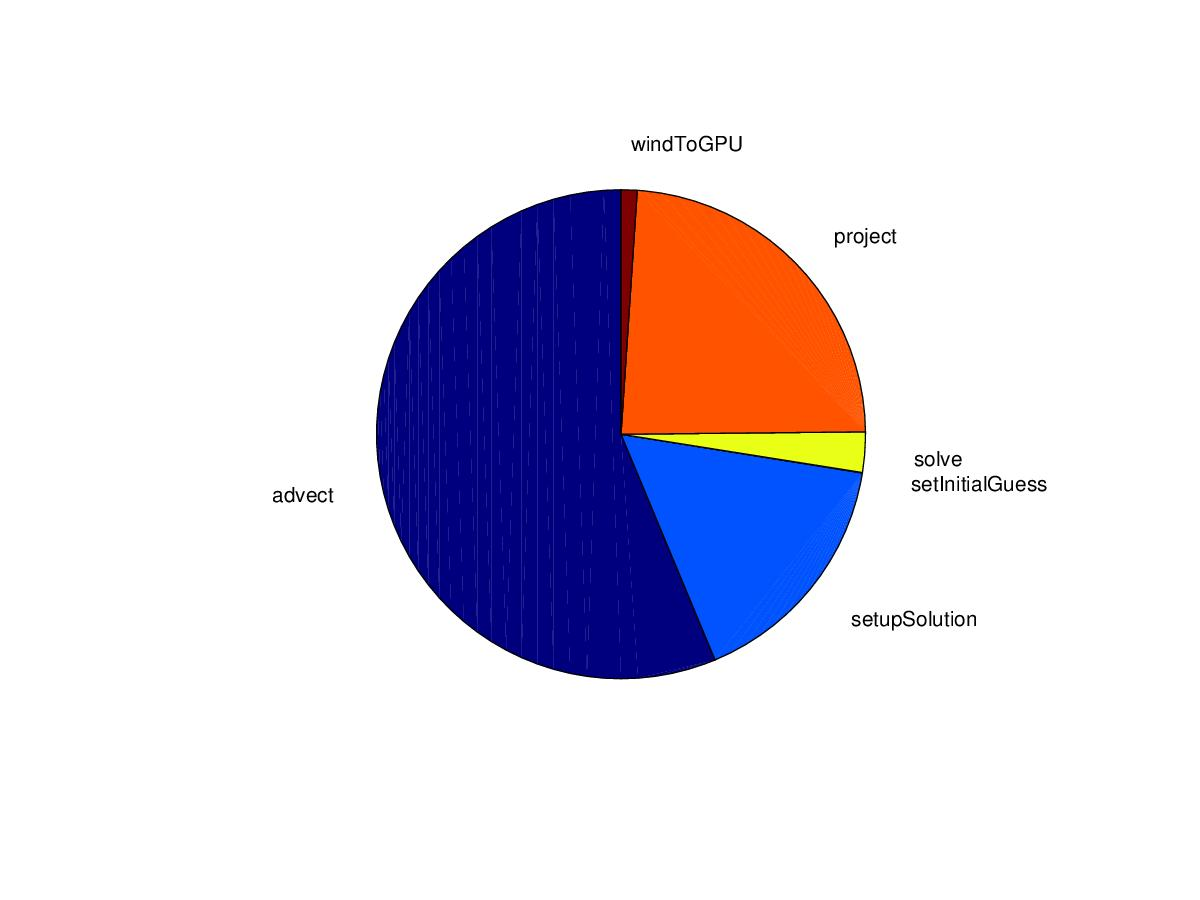
\includegraphics[width=1.0\textwidth]{results/data/td_conf3_petsc_gpu}
		\caption{PETSc on the GPU with OpenCL.}
		\label{fig:td_conf3_petsc_gpu}
	\end{subfigure}
	\begin{subfigure}{0.45\textwidth}
		\center
		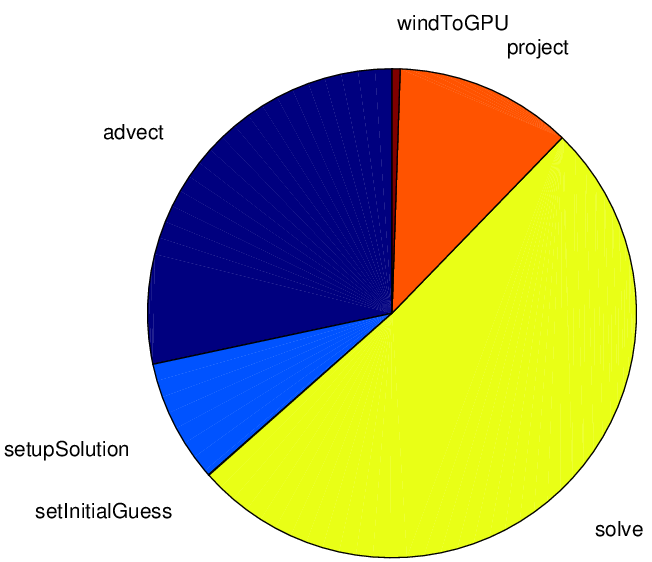
\includegraphics[width=1.0\textwidth]{results/data/td_conf3_petsc_cpu}
		\caption{PETSc on the CPU.}
		\label{fig:td_conf3_petsc_cpu}
	\end{subfigure}
	\caption{Time distribution of the execution time of the key functions
			with configuration 3}
	\label{fig:td_conf3}
	
\end{figure}

\begin{figure}[ht]
	\center
	
	\begin{subfigure}{0.45\textwidth}
		\center
		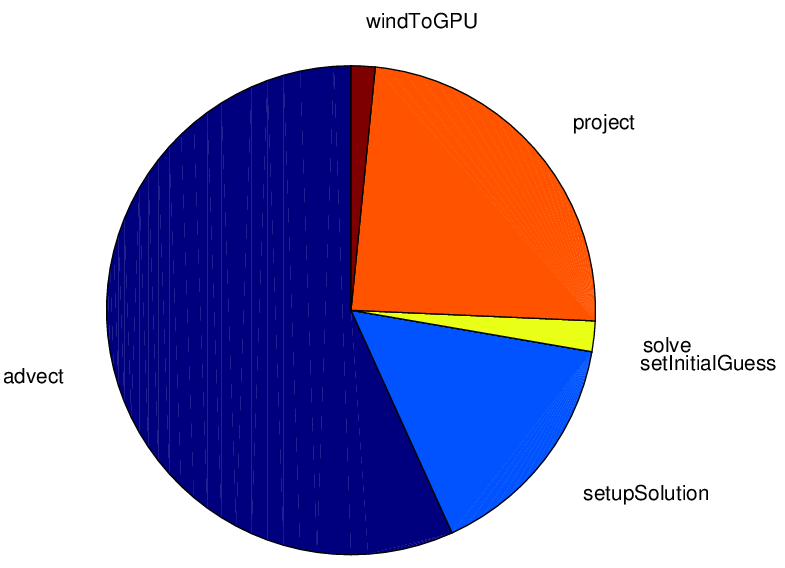
\includegraphics[width=1.0\textwidth]{results/data/td_conf4_petsc_gpu}
		\caption{PETSc on the GPU with OpenCL.}
		\label{fig:td_conf4_petsc_gpu}
	\end{subfigure}
	\begin{subfigure}{0.45\textwidth}
		\center
		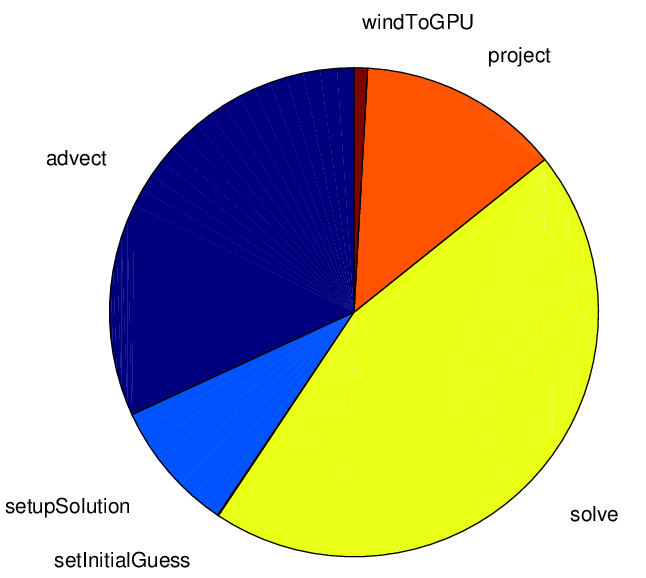
\includegraphics[width=1.0\textwidth]{results/data/td_conf4_petsc_cpu}
		\caption{PETSc on the CPU.}
		\label{fig:td_conf4_petsc_cpu}
	\end{subfigure}
	\caption{Time distribution of the execution time of the key functions
			with configuration 4}
	\label{fig:td_conf4}
	
\end{figure}

As evident from these charts we can see that as the resolution of the wind
velocity field increases, the fraction of the wind simulation time spent solving
the Poisson equation remains roughly unchanged for the PETSc on CPU only
implementation, however when the GPU is utilized for the solver the fraction of
the simulation time spent solving the Poisson equation is reduced rapidly as
the computational power of the GPU is better utilized for larger problems because
of the GPU's parallel nature.

\subsection{Visual Results}

TODO: Show the windfield and pressure field and obstacle field (if I have time)


\clearpage

\chapter{Discussion}

\clearpage

\chapter{Conclusion}

In this project PETSc has been used to implement a wind simulator for the HPC-
lab's snow simulator. This was done to investigate the performance gain
obtainable by using high level libraries to use the GPU for computationally
intensive problems instead of hand implementing solvers with low level APIs like
CUDA and OpenCL. A PETSc implementation enables easy experimentation with
parallelization method as PETSc supports shared memory parallelization,
distributed memory parallelization and GPGPU. In addition PETSc implements a
large number of solvers making it easy to experiment with the choice of solver
for the wind simulator.

The results show that using the GPU implementation of PETSc gives large speedups
for the solver without having to make special adjustments to the code to account
for the GPU. PETSc's GPU implemented solvers can achieve performance comparable
to that of hand tuned implementations written in low level APIs like CUDA and
OpenCL.

A drawback with PETSc is that it is challenging to use for
operations that are not straight forward to define using functions implemented
in PETSc. For example trilinear interpolation required for the advection step of
the wind simulation. Because of this only the implementation of the Poisson
solver uses the GPU for computation in this project. This severely limits the
size of the wind velocity field for the wind simulation.

Further more, configuring PETSc to use CUDA can be very challenging because of
issues with backwards compatibility. Using PETSc with CUDA could require running
the application on old GPU hardware, or updating PETSc itself to resolve the
backwards compatibility issues.

\clearpage

\chapter{Future Work}

\section{Parallelization}

\clearpage

\begin{appendices}

\chapter{Abbreviations}

\begin{description}
	\item[PDE] Partial Differential Equation
	\item[FDM] Finite Difference Method
\end{description}


\chapter{Linking PETSc}

The following Cmake modules from Jed Brown's \emph{cmake-modules}
\footnote{\url{https://github.com/jedbrown/cmake-modules}}
github was added to the project. These modules are distributed under the BSD 2-Clause
license. 

\begin{itemize}
	\item CorrectWindowsPaths.cmake
	\item FindPETSc.cmake
	\item FindPackageMultipass.cmake
	\item ResolveCompilerPaths.cmake
\end{itemize}

\end{appendices}

\clearpage

\bibliography{bibliography}
\clearpage

\end{document}
